\documentclass[11pt]{article}
\usepackage[margin=1in]{geometry}
\usepackage{amsmath,amssymb,amsthm,mathtools}
\usepackage{graphicx}
\usepackage{enumitem}
\usepackage[hidelinks]{hyperref}
\usepackage{microtype}

\newtheorem{theorem}{Theorem}
\newtheorem{lemma}[theorem]{Lemma}
\newtheorem{remark}[theorem]{Remark}
\newcommand{\Ban}{\mathbf{Ban}}
\newcommand{\CMet}{\mathbf{CMet}}
\newcommand{\F}{\mathbb F}
\newcommand{\N}{\mathbb N}

\title{Enriched Finitely Presentable Banach Spaces\\
Are Exactly the Finite-Dimensional Ones}
\author{Discovery packet for arXiv:2206.08546\\
\texttt{fa\_banach\_001}, lane 17, \texttt{agent\_lane\_17}}
\date{11 August 2026}

\begin{document}
\maketitle

\begin{center}
\fbox{\parbox{0.92\textwidth}{
\textbf{Status.} Candidate full solution, likely valid, requiring expert
review.  A single fixed sequential diagram on $c_0$ detects every
infinite-dimensional Banach space.  Josefson--Nissenzweig supplies the
obstructing morphism, and the left-shift tails violate the exact hom-metric
condition for enriched finite presentability.
}}
\end{center}

\section{Source and exact question}

Let $\Ban$ be the category of real or complex Banach spaces and linear
contractions, enriched over complete metric spaces by the operator-norm
metric on each hom-set.  In Ji\v{r}\'i Rosick\'y,
\emph{Enriched purity and presentability in Banach spaces},
arXiv:2206.08546 and \emph{Communications in Algebra} 51 (2023),
5242--5262 \cite{Rosicky}, Theorem 3.1 proves that every finite-dimensional
Banach space is finitely presentable in this enriched sense.

Remark 3.3 then asks for the converse: must every enriched finitely
presentable Banach space be finite-dimensional?  The answer is yes.  In fact,
the converse is witnessed by one countable diagram, independent of the
Banach space.

\begin{figure}[p]
  \centering
  
\includegraphics[width=\textwidth]{figures/open_problem_page8.png}
  \caption{Source page 8.  Remark 3.3 states the finite-dimensionality
  question after recalling the two hom-metric conditions for preservation of
  directed colimits.}
\end{figure}
\clearpage

\section{Full result}

Write $c_0=c_0(\F)$ and let
\[
 S:c_0\longrightarrow c_0,\qquad
 S(a_1,a_2,a_3,\ldots)=(a_2,a_3,a_4,\ldots)
\]
be the left shift.  Consider the fixed sequential directed diagram
\begin{equation}\label{eq:shift-diagram}
 \mathcal D:\qquad
 c_0\xrightarrow{S}c_0\xrightarrow{S}c_0\xrightarrow{S}\cdots .
\end{equation}

\begin{theorem}[Classification and a universal detector]\label{thm:main}
For a real or complex Banach space $A$, the following are equivalent.
\begin{enumerate}[label=\textnormal{(\roman*)}]
\item $A$ is finite-dimensional.
\item $A$ is finitely presentable in the $\CMet$-enriched category $\Ban$.
\item The enriched representable functor
\[
 \Ban(A,-):\Ban\longrightarrow\CMet
\]
preserves the colimit of the single diagram $\mathcal D$ in
\eqref{eq:shift-diagram}.
\end{enumerate}
\end{theorem}

Thus Remark 3.3 has a positive answer.  The strengthening in (iii) says that
no diagram depending on $A$ is needed.

\section{The two ingredients}

\begin{lemma}[The shift diagram has zero colimit]\label{lem:colimit}
The colimit of $\mathcal D$ in $\Ban$ is the zero Banach space.
\end{lemma}

\begin{proof}
The zero maps form a cocone.  Let $(u_n:c_0\to E)_{n\geq0}$ be any other
cocone of contractions, so
\[
 u_n=u_{n+m}S^m\qquad(n,m\geq0).
\]
For $z\in c_0$,
\[
 \|u_nz\|=\|u_{n+m}S^mz\|\leq\|S^mz\|\longrightarrow0
 \qquad(m\to\infty).
\]
Hence every $u_n$ is zero.  The zero cocone is therefore universal.
\end{proof}

\begin{lemma}[An infinite-dimensional witness]\label{lem:witness}
If $A$ is infinite-dimensional, there is a contraction $J:A\to c_0$ such
that
\begin{equation}\label{eq:tails}
 \|S^mJ\|=1\qquad(m\geq0).
\end{equation}
\end{lemma}

\begin{proof}
The Josefson--Nissenzweig theorem gives a sequence
$(\varphi_r)_{r\geq1}\subset A^*$ such that
\[
 \|\varphi_r\|=1\quad\hbox{for every }r,
 \qquad
 \varphi_r(x)\longrightarrow0\quad\hbox{for every }x\in A
\]
\cite{Josefson,BanakhGabriyelyan}.  Define
\[
 Jx=(\varphi_1(x),\varphi_2(x),\ldots).
\]
Pointwise nullity makes $Jx\in c_0$, and
\[
 \|J\|=\sup_{r\geq1}\|\varphi_r\|=1.
\]
For every $m\geq0$,
\[
 \|S^mJ\|
 =\sup_{\|x\|\leq1}\sup_{r>m}|\varphi_r(x)|
 =\sup_{r>m}\|\varphi_r\|=1,
\]
which is \eqref{eq:tails}.
\end{proof}

\begin{figure}[p]
  \centering
  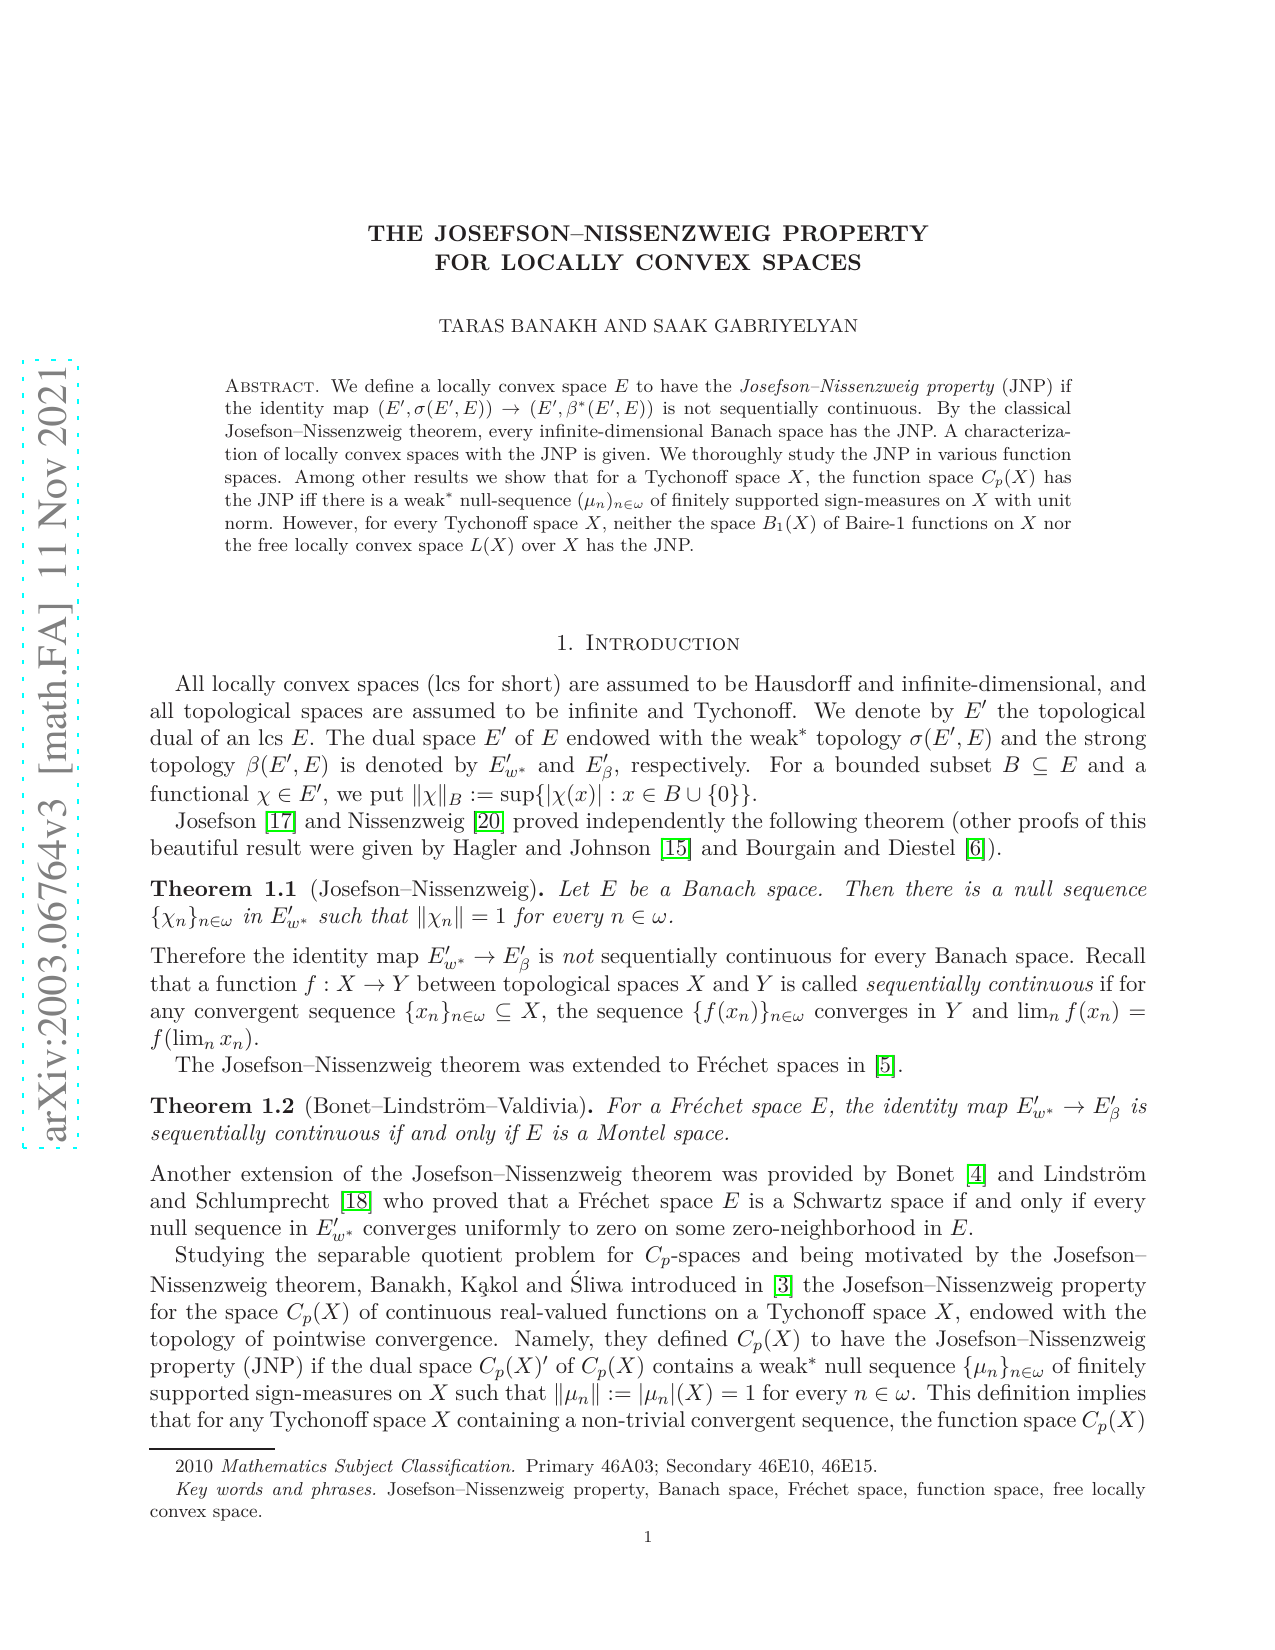
\includegraphics[width=0.96\textwidth]{figures/jn-01.png}
  \caption{A modern statement of the Josefson--Nissenzweig theorem:
  Theorem 1.1 in Banakh--Gabriyelyan \cite{BanakhGabriyelyan}.}
\end{figure}
\clearpage

\section{Proof of Theorem~\ref{thm:main}}

The implication (i)$\Rightarrow$(ii) is Rosick\'y's Theorem 3.1
\cite{Rosicky}.  The implication (ii)$\Rightarrow$(iii) is immediate from
the definition of enriched finite presentability.

It remains to prove (iii)$\Rightarrow$(i).  We argue contrapositively.
Suppose $A$ is infinite-dimensional and choose $J$ from
Lemma~\ref{lem:witness}.  Applying $\Ban(A,-)$ to $\mathcal D$ gives the
sequential diagram of complete metric spaces
\[
 \Ban(A,c_0)\xrightarrow{S\circ-}\Ban(A,c_0)
 \xrightarrow{S\circ-}\Ban(A,c_0)\xrightarrow{S\circ-}\cdots .
\]
For a directed colimit of metric spaces, the distance between two elements
represented at the same stage is the infimum of their distances at all later
stages (followed by the usual zero-distance quotient and completion).
Consequently, the distance in this colimit between the stage-zero classes of
$J$ and $0$ is
\[
 \inf_{m\geq0}\|S^mJ-S^m0\|
 =\inf_{m\geq0}\|S^mJ\|=1.
\]
In particular, this metric colimit is not a singleton.

On the other hand, Lemma~\ref{lem:colimit} says
$\operatorname*{colim}\mathcal D=0$ in $\Ban$, and hence
\[
 \Ban\!\left(A,\operatorname*{colim}\mathcal D\right)
 =\Ban(A,0)
\]
is a singleton.  The canonical comparison from the preceding metric colimit
to $\Ban(A,0)$ collapses the two points represented by $J$ and $0$, which
remain distance one apart.  It is not an isomorphism in $\CMet$.  Thus
$\Ban(A,-)$ does not preserve this colimit, contradicting (iii).
Therefore $A$ is finite-dimensional.

\begin{remark}[The source's condition (2) fails as sharply as possible]
Let $k_0:c_0\to0$ be the colimit map.  Taking $f=J$ and $g=0$ at stage zero,
the equality required in condition (2) on source page 6 is
\[
 \|k_0f-k_0g\|
 =\inf_{m\geq0}\|S^mf-S^mg\|.
\]
The left side is $0$, while the right side is $1$.  There is no limiting or
completion subtlety: the defect is maximal and persists at every stage.
\end{remark}

\section{Why the shift is the exact detector}

The finite-dimensional and infinite-dimensional cases are separated by
uniformity on the unit ball.

If $A$ is finite-dimensional and $T:A\to c_0$ is bounded, then
$S^mTx\to0$ for each $x$.  On the compact unit ball of $A$, the continuous
functions
\[
 q_m(x)=\|S^mTx\|
\]
decrease pointwise to zero.  Dini's theorem gives
$\|S^mT\|=\sup_{\|x\|\leq1}q_m(x)\to0$.  Thus every pair of morphisms becomes
identified in the $\CMet$-colimit of the represented shift diagram.

For infinite-dimensional $A$, Josefson--Nissenzweig is precisely the failure
of that uniformity: the pointwise-null sequence $(\varphi_r)$ has unit norms.
Packaging the sequence as $J:A\to c_0$ converts nonuniform weak-star nullity
into the persistent tail equality $\|S^mJ\|=1$.  This explains why the same
diagram works for all $A$ and why neither separability nor a basis nor an
approximation property is required.

\section{Proof and upgrade audit}

Eight routes or possible failure modes were checked.

\begin{enumerate}[leftmargin=*,label=\textbf{Route \arabic*.}]
\item The Josefson--Nissenzweig sequence was packaged as an operator into
$c_0$ and paired with the left shift.  This gives the full solution.

\item A scalar contraction chain was tested first.  Although its Banach
colimit is zero, the norms of every represented morphism also decay, so it
cannot violate the hom-metric equality.

\item Tail projections associated to a Schauder basis give the right
phenomenon for spaces with a basis, but do not cover arbitrary Banach spaces.
Josefson--Nissenzweig removes this restriction.

\item A basic-sequence construction was tested.  It lives naturally on a
subspace and requires noncanonical extension control; the global weak-star
null sequence is the correct replacement.

\item Quotients by increasing finite-dimensional pieces were considered.
They do not give a universal sequential exhaustion in nonseparable spaces.
The fixed $c_0$ shift avoids all density-character issues.

\item The zero-colimit claim was checked directly by the universal property,
not merely by the usual seminorm formula.

\item The $\CMet$ colimit was checked at the level of its exact pseudometric:
$J$ and $0$ retain distance one before quotienting and completion, so they
cannot be accidentally identified.

\item Both real and complex scalars were audited.  Josefson--Nissenzweig,
$c_0(\F)$, the shift, and the norm computation work in either case.
\end{enumerate}

\section{Novelty bounds and recommendation}

The four lightweight run indexes were searched for arXiv:2206.08546, the
paper title, enriched finite presentability, the exact Remark 3.3 phrasing,
Josefson--Nissenzweig, and the $c_0$ shift; no prior run result was found.

A bounded Crossref/OpenAlex audit identified the published source DOI
\url{https://doi.org/10.1080/00927872.2023.2228412} and exactly two citing
works as of
11 August 2026.  Chirvasitu \cite{Chirvasitu} gives an alternative proof of
the finite-dimensional positive direction, but does not discuss the converse.
Rosick\'y--Tendas \cite{RosickyTendas} develops notions of enriched purity,
but likewise gives no finite-presentability classification.  Full texts of
both citing papers were searched for the exact question, finite-dimensional
converses, Josefson--Nissenzweig, and shift arguments.  Bounded web/arXiv
queries found the source and the standard Josefson--Nissenzweig literature,
but no direct answer.  This is not an exhaustive literature certification.

Human review should focus on only three points: the universal property in
Lemma~\ref{lem:colimit}, the exact tail norm in Lemma~\ref{lem:witness}, and
the standard directed-colimit metric formula used in the final comparison.
If accepted, the argument is a short full answer to Remark 3.3 and the
fixed-diagram strengthening should be recorded with it.

\begin{thebibliography}{9}

\bibitem{Rosicky}
J. Rosick\'y,
\emph{Enriched purity and presentability in Banach spaces},
Communications in Algebra 51 (2023), 5242--5262,
DOI \texttt{10.1080/00927872.2023.2228412}.

\bibitem{Josefson}
B. Josefson,
\emph{Weak sequential convergence in the dual of a Banach space does not
imply norm convergence},
Arkiv f\"or Matematik 13 (1975), 79--89,
DOI \texttt{10.1007/BF02386198}.

\bibitem{BanakhGabriyelyan}
T. Banakh and S. Gabriyelyan,
\emph{The Josefson--Nissenzweig property for locally convex spaces},
Filomat 37 (2023), 2517--2529,
DOI \texttt{10.2298/FIL2308517B}; arXiv:2003.06764.

\bibitem{Chirvasitu}
A. Chirvasitu,
\emph{Semisimplicity manifesting as categorical smallness},
Theory and Applications of Categories 41 (2024), 470--492,
DOI \texttt{10.70930/tac/ixrw9w9v}.

\bibitem{RosickyTendas}
J. Rosick\'y and G. Tendas,
\emph{Notions of enriched purity},
Theory and Applications of Categories 41 (2024), 2058--2104,
DOI \texttt{10.70930/tac/da0gvaco}.

\end{thebibliography}

\end{document}
